\RequirePackage{luatex85}
\documentclass[tikz, border=10pt]{standalone}

\usepackage[compat=1.1.0]{tikz-feynman}

\begin{document}

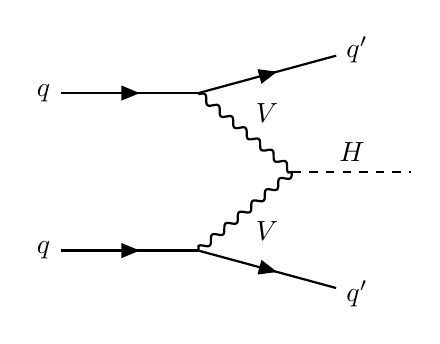
\begin{tikzpicture}[thick]
 \begin{feynman}
  \vertex (origin);
  \vertex [right=1.5cm of origin] (H);
  \vertex [above left=1cm and 1.2cm of origin] (v1);
  \vertex [below left=1cm and 1.2cm of origin] (v2);
  \vertex [left=1.75cm of v1] (q1) {\(q\)};
  \vertex [left=1.75cm of v2] (q2) {\(q\)};
  \vertex [above right=0.25cm and 1.75cm of v1] (q3) {\(q'\)};
  \vertex [below right=0.25cm and 1.75cm of v2] (q4) {\(q'\)};
  \diagram* {
  (v1) -- [boson, edge label={\(V\)}] (origin),
  (origin) -- [boson, edge label={\(V\)}] (v2),
  (origin) -- [scalar, edge label={\(H\)}] (H),
  (q1) -- [fermion] (v1),
  (q2) -- [fermion] (v2),
  (v1) -- [fermion] (q3),
  (v2) -- [fermion] (q4),
  };
 \end{feynman}
\end{tikzpicture}
\end{document}
